\section{Stetigkeit}
  \begin{definition}
    \textbf{A:} \newline Eine Funktion $f:D\rightarrow \R$ mit $D \subset \R$ heißt stetig in $x^* \in D$, falls $\lim\limits_{x \rightarrow x^*} f(x) = f(x^*)$. \label{def:stet_a}
  \end{definition}
  \begin{bem}
    Jede in $x^*$ differenzierbare Funktion ist auch stetig in $x^*$.
  \end{bem}
  \begin{definition}
    Eine Funktion $f:D\rightarrow \R$ mit $D \subset \R$ heißt stetig, falls $f$ stetig für alle $x^* \in D$ ist.
  \end{definition}
  \begin{satz}
    Sind $f$, $g$ stetige Funktionen und $\lambda \in \R$, so sind innerhalb ihres Definitionsbereich auch $\lambda f$, $f+g$, $f\cdot g$, $f\circ g$, $\frac{f}{g}$ stetige Funktionen.
  \end{satz}
  \begin{satz}
  Stetige Fortsetzbarkeit: Eine Definitionslücke einer gebrochen rationalen Funktion ist hebbar, wenn die Vielfachheit der Nullstelle $x_0$ im Zäherpolynom $\geq$ der Vielfachheit der Nullstelle $x_0$ im Nennerpolynom ist.
  \end{satz}
  \subsection{Arten von Unstetigkeiten}
  \begin{figure}[H] 
		\centering
		\begin{minipage}{.5\textwidth}
		  \centering
		  \captionsetup{justification=centering}
		  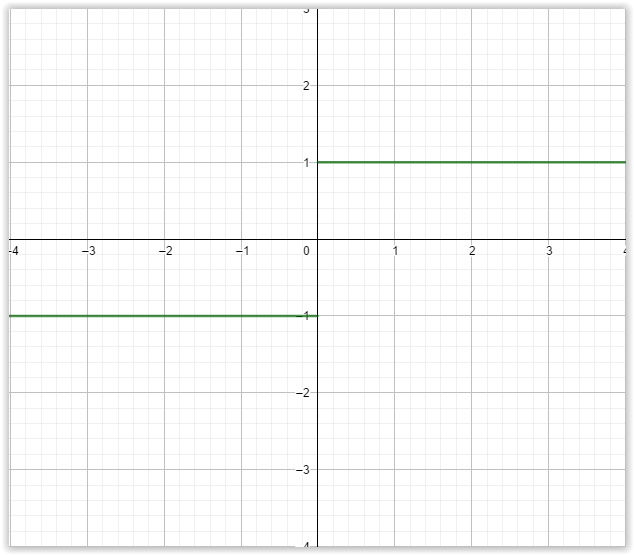
\includegraphics[width=0.78\linewidth]{./img/stetigkeit_sprung.png}
		  \caption{$f(x) = \frac{|x|}{x}$ \\ (Sprungstelle)}
		  \label{fig:stetigkeit_sprung}
		\end{minipage}%
		\begin{minipage}{.5\textwidth}
		  \centering
		  \captionsetup{justification=centering}
		  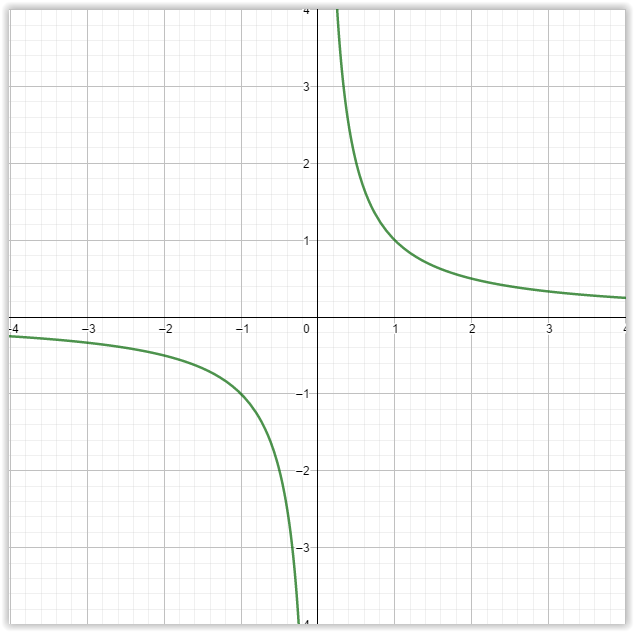
\includegraphics[width=0.7\linewidth]{./img/stetigkeit_pol.png}
		  \caption{$f(x) = \frac{1}{x}$ \\ (Polstelle)}
		  \label{fig:stetigkeit_pol}
		\end{minipage}
  \end{figure}
  \begin{figure}[H] 
		\centering
	  \centering
	  \captionsetup{justification=centering}
	  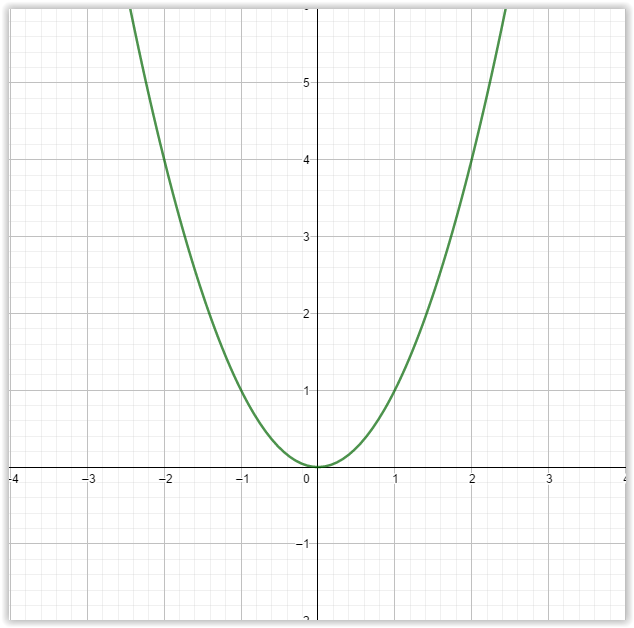
\includegraphics[width=0.35\linewidth]{./img/stetigkeit_luecke.png}
	  \caption{$f(x) = \frac{x^3}{x}$ \\ (Lücke)}
	  \label{fig:stetigkeit_luecke}
  \end{figure}
  \begin{definition}
    $f:D\rightarrow \R$, $f(x)$ ist stetig in $x_0 \in D$ falls \newline
    \begin{itemize}
      \item[1) ] Falls z.z. ist dass $f$ stetig ist:
      \begin{equation}
        \forall \varepsilon > 0 \quad \exists \delta_\varepsilon \quad \forall x \in D: \left(|x-x_0| < \delta_\varepsilon \Rightarrow |f(x) - f(x_0)| < \varepsilon \right)
      \end{equation}
      \item[2) ] Falls z.z. ist dass $f$ nicht stetig ist:
      \begin{equation}
        \forall \text{ Folgen } (x_n) \text{ mit }x_n \rightarrow x_0 \text{ für }n \rightarrow \infty \Rightarrow f(x_n) \rightarrow f(x_0) \text{ für } n \rightarrow \infty.
      \end{equation}
      \item[2) ] 
      \begin{equation}
        \lim\limits_{x \rightarrow x_o^-} f(x) = \lim\limits_{x \rightarrow x_o^+} f(x)
        \end{equation}
    \end{itemize}
  \end{definition}
  \subsection{Nullstellensatz und Zwischenwertsatz}
  \begin{satz}
    Es sei $f: [a,b]\rightarrow \R§$ eine stetige Funktion. Dann gilt:
    \begin{itemize}
      \item[a) ] Es sei $f(a)f(b) < 0$. Dann existiert ein $x^*\in(a,b)$ mit $f(x^*) = 0$, d.h. eine Nullstelle von $f$.
      \item[b) ] Sei $f(a) < c < f(b)$. Dann existiert ein $x^* \in (a,b)$ mit $f(x^*) = c$.
    \end{itemize}
    \begin{figure}[H] 
			\centering
			\begin{minipage}{.5\textwidth}
			  \centering
			  \captionsetup{justification=centering}
			  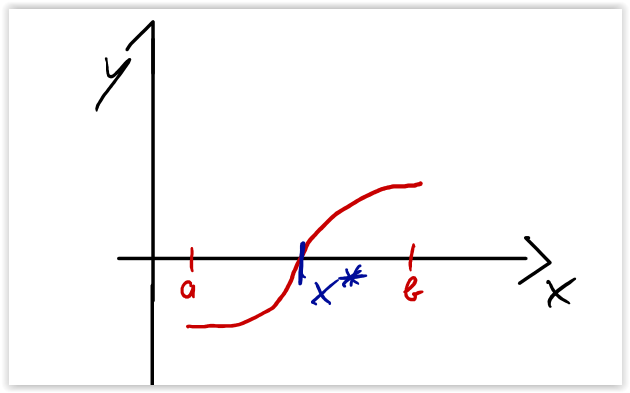
\includegraphics[width=0.75\linewidth]{./img/potenzreihen_nullstellensatz.png}
			  \caption{Zu a) \\ (Nullstellensatz) \protect\cite{HM12}}
			  \label{fig:reihe_potenzradius_r}
			\end{minipage}%
			\begin{minipage}{.5\textwidth}
			  \centering
			  \captionsetup{justification=centering}
			  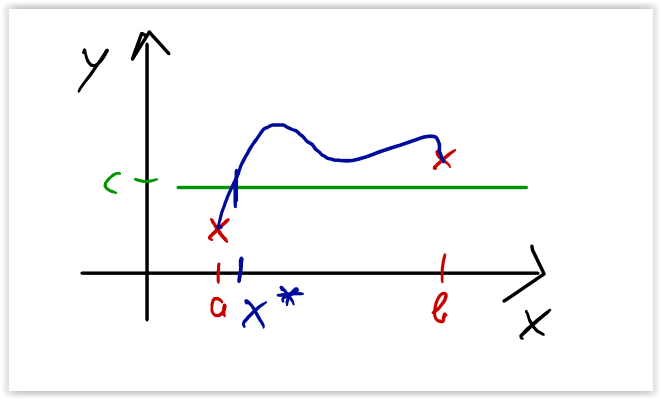
\includegraphics[width=0.8\linewidth]{./img/potenzreihen_zwischenwertsatz.png}
			  \caption{Zu b) \\ (Zwischenwertsatz) \protect\cite{HM12}}
			  \label{fig:reihe_potenzradius_c}
			\end{minipage}
    \end{figure}
  \end{satz}
  \subsubsection{Sätze zu Stetigkeit und Monotonie}
  \begin{satz}
    $f:[a,b] \rightarrow \R$ sei streng monoton wachsend und  stetig. Dann existiert die Umkehrfunktion $f^{-1}:[f(a),f(b)]\rightarrow \R$. Diese ist streng monoton wachsend und stetig.
  \end{satz}
  \begin{definition}
    \textbf{B: ($\varepsilon -\delta$ Definition)} \newline
    Se $f:D\rightarrow \R$ mit $D \subset \R$. Dann heißt $f$ stetig in $x^*$, wenn für alle $\varepsilon > 0$ ein $\delta > 0$ existiert, sodass gilt: 
    \begin{equation}
      \forall x \in D:\quad |x - x^*| < \delta \Rightarrow |f(x) - f(x^*)| < \varepsilon
    \end{equation}
    Es muss zu jeder beliebig kleinen Seitenlänge $\varepsilon$ immer ein Rechteck mit Mitte $x^*$ existieren, sodass $f$ das Rechteck an den Seiten verlässt.
    \begin{figure}[H] 
			\centering
			\captionsetup{justification=centering}
			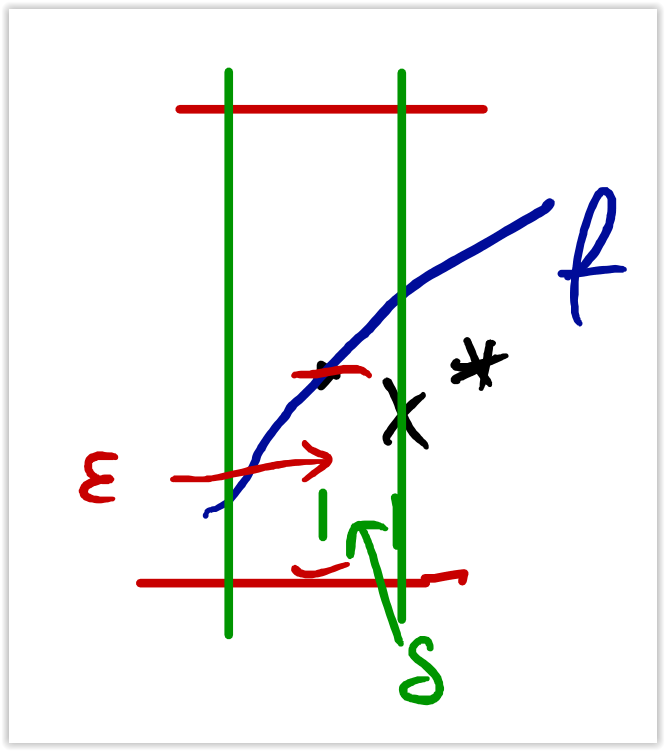
\includegraphics[width=0.2\linewidth]{./img/stetigkeit_eps_del.png}
			\caption{$\varepsilon - \delta$ Kriterium \protect\cite{HM12}}
			\label{fig:stetigkeit_eps_del}
    \end{figure} \label{def:stet_b}
  \end{definition}
  
  \begin{definition}
    \begin{itemize}
      \item[a) ] $f$ heißt Lipschitz-stetig in $x^*$, wenn es ein $L > 0$ und $\delta > 0$ gibt, sodass für $x \in D$ mit $|x-x^*| < \delta$
	      \begin{equation}
	        |f(x) - f(x^*) \leq L|x-x^*|
	      \end{equation}
	      gilt.
      \item[b) ] $f$ heißt Hölder-stetig mit Exponent $\alpha \in (0,1]$, falls
	      \begin{equation}
	        |f(x) - f(x^*)| \leq L(|x-x^*|^\alpha
	      \end{equation}
	      gilt.
    \end{itemize}
    \begin{figure}[H] 
			\centering
			\begin{minipage}{.5\textwidth}
			  \centering
			  \captionsetup{justification=centering}
			  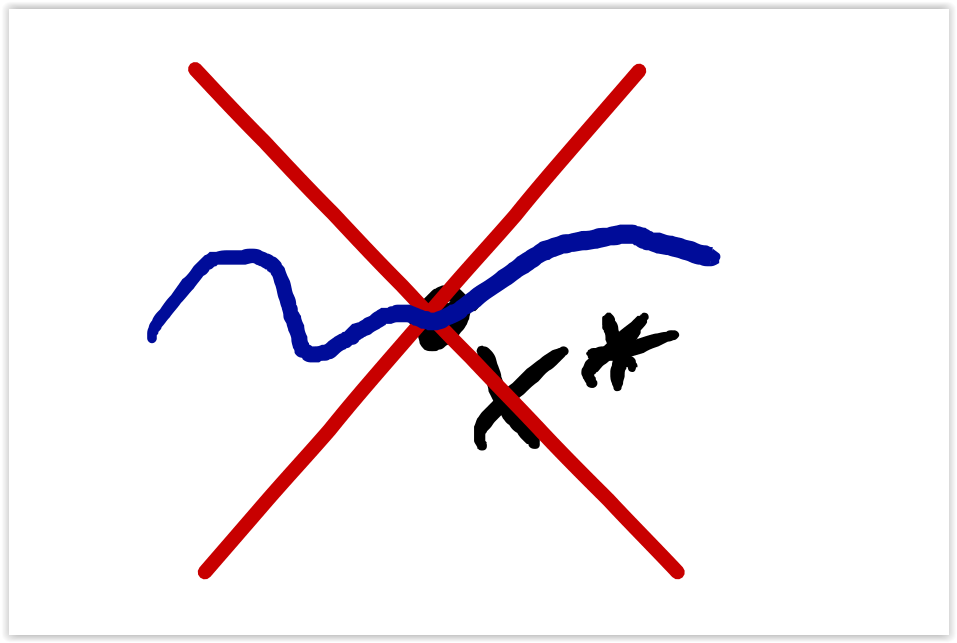
\includegraphics[width=0.9\linewidth]{./img/stetigkeit_lipschitz.png}
			  \caption{Zu a) \\ (Lipschitzstetigkeit) \protect\cite{HM12}}
			  \label{fig:stetigkeit_lipschitz}
			\end{minipage}%
			\begin{minipage}{.5\textwidth}
			  \centering
			  \captionsetup{justification=centering}
			  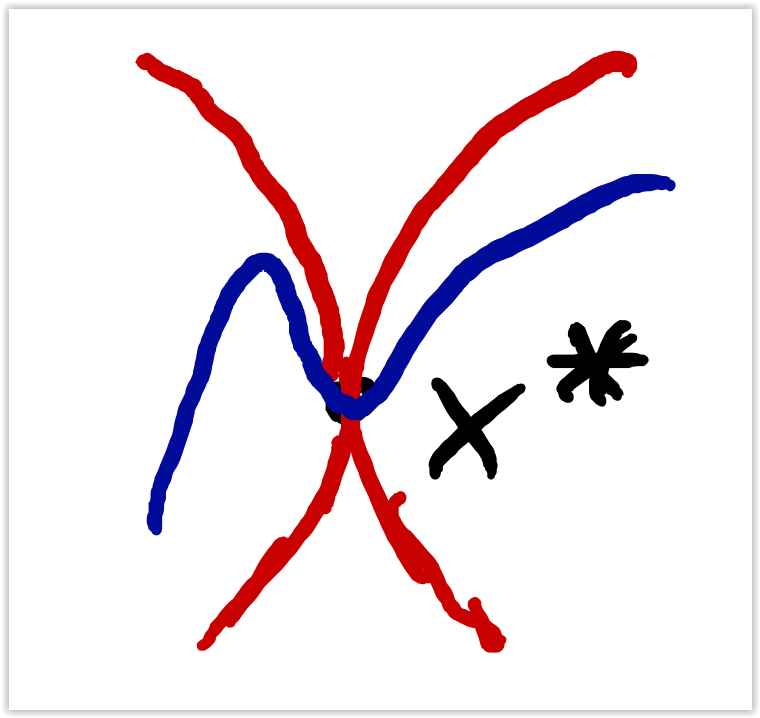
\includegraphics[width=0.65\linewidth]{./img/stetigkeit_hoelder.png}
			  \caption{Zu b) \\ (Hölder-Stetigkeit) \protect\cite{HM12}}
			  \label{fig:stetigkeit_hoelder}
			\end{minipage}
    \end{figure}
  \end{definition}
  \begin{bem}
  \textbf{Zu a)}
    Es ist die Idee, eine Sekante so in den Graph zu legen, dass sie zwei Punkte des Graphen schneidet. Existiert nun eine Sprungstelle, so kann man diese Bedingung einhalten und die Steigung der Sektanten gegen unendlich treiben (praktisch eine senkrechte gerade). Liegt keine Sprungstelle vor, so wird die Steigung unter Einhaltung der Bedingung immer kleiner unendlich sein. Die Schranke für die Steigung ist hier $L$.
  \end{bem}
  \begin{satz}
    Definition A \eqref{def:stet_a} und Definition B \eqref{def:stet_b} der Stetigkeit sind äquivalent.
  \end{satz}
  \begin{definition}
    Eine Funktion $f:D\rightarrow \R$ mit $D \subset \R$ heißt Hölder- bzw. Lipschitzstetig, falls $f$ Hölder- bzw. Lipschitzstetig in jedem $x^* \in D$ ist. \newline
    Bezeichnungen: $C^{0,\alpha}$ steht für Hölder-stetig, $C^{0,1} = Lip$ steht für Lipschitzstetig.
  \end{definition}
  \begin{bem}
    Es gilt:
    \begin{equation}
      \text{differenzierbar } \Rightarrow \text{Lipschitzstetig } \Rightarrow \text{Hölder-stetig } \Rightarrow \text{stetig }
    \end{equation}
  \end{bem}    
  \newpage 
  